\documentclass{article}
\usepackage{geometry}
\usepackage{paralist}
\usepackage[T1]{fontenc}
\usepackage{reledmac}
\usepackage{changepage}
\usepackage{layout}

\usepackage{pgfplots}
\usepackage{tikz}
\usetikzlibrary{positioning}
\usetikzlibrary{shapes.geometric, arrows}
\usetikzlibrary{calc, shapes, backgrounds}
\tikzstyle{arrow} = [thick,->,>=stealth]

\usepackage{graphicx} 
\graphicspath{ {./images/} }

\usepackage{fancyhdr}
\fancyhead[L]{
	\begin{tabular}{l}
		\Large \textbf{\textsc{Advanced Networking and Future Internet}} \\
		\large Theoretical Exercise 09
	\end{tabular}
}
\fancyhead[R]{
	\begin{tabular}{r}
		16-124-836 \\
		Marcel \textsc{Zauder}
	\end{tabular}
}
\renewcommand{\headrulewidth}{0.4pt}
\fancyfoot[C]{\thepage}
\renewcommand{\footrulewidth}{0.4pt}
\setlength{\headsep}{35pt}
\setlength{\textheight}{600pt}

\usepackage{hyperref}

\begin{document}
	\pagestyle{fancy}
	
	\section*{9.1 Uncompressed Audio \& Video}
	\begin{adjustwidth}{2em}{2em}
		\begin{enumerate}
			\item \textbf{Audio}
			\begin{adjustwidth}{-2em}{}
			\begin{tabular}{|c|c|c|c|}
				\hline
				\textbf{Quality} & \textbf{Sample Rate (kHz)} & \textbf{Quantization Level} & \textbf{Bandwidth (Mbps)} \\
				\hline
				AM Radio (stereo) & 11.025 & 8 & 0.1764 Mbps \\
				FM Radio (stereo) & 22.05 & 16 & 0.7056 Mbps \\
				HD/DVD Audio & 192 & 24 & 4.608 Mbps \\
				\hline
			\end{tabular}
			\end{adjustwidth}
			\item \textbf{Video} \\
			\begin{tabular}{|c|c|c|c|c|}
				\hline
				\textbf{Quality} & \textbf{Resolution} & \textbf{Bits Per Pixel} & \textbf{FPS} & \textbf{Bandwidth (Mbps/Gbps)} \\
				\hline
				4k Video & 3840 x 2160 & 24 & 24 & 4'777.574 Mbps / 4.777 Gbps \\
				5k Video & 5140 x 2880 & 36 & 30 & 15'987.456 Mbps / 15.987 Gbps \\
				8k Video & 7680 x 4320 & 48 & 60 & 95'551.488 Mbps / 95.551 Gbps \\
				\hline
			\end{tabular}
		\end{enumerate}
	\end{adjustwidth}
	
	\section*{9.2 Digitization of Audio Data}
	\begin{adjustwidth}{2em}{2em}
		\subsection*{9.2.1 Explain (in detail!) the steps required to transmit audio data over a network}
		\begin{adjustwidth}{2em}{2em}
			In total the analogue data is transformed into digital data, then transmitted over the network and at the end transformed back to analog data. \\
			First an AD-Converter is used to change the analogue data to a digital data type. This Converter takes the continous-time and continous-amplitude signal and converts it to discrete-time and discrete-amplitude-signals. The amplitude is measured periodically and is depending on the sample rate (for example 69kHz is 69000 samples per second). To get the best result the sampling rate should be greater than 2 times the highest occuring frequency (sampling theorem). Such the signal by using the sampling and the quantization (assigning a numerical value to a sample) is encoded. The higher the amount of available bits for sending the higher the resolution is. \\
			This digitalized signal can now be transmitted and with the information the receiver can transform this digital data back to the analogue data with a similar DA-Converter.
		\end{adjustwidth}
		\subsection*{9.2.2 What is meant by the term Aliasing?}
		\begin{adjustwidth}{2em}{2em}
			Aliasing is an effect which occurs when encoding a signal. It causes a signal to become indistinguishable from other signals when being sampled. We take the following image as an example:
			\begin{center}
			\includegraphics[scale=0.6]{Aliasing.jpg}			
			\end{center}
			We wanted to encode the red frequence but when decoding the blue signal is created. As we can see the possibility of aliasing is increased when the sampling rate is too low and therefore the encoding for the red and blue signals are the same; they are aliases from one another. In this case we cannot distinguish between which signal was the source of our encoiding.
		\end{adjustwidth}
		\subsection*{9.2.3 How can Aliasing be corrected?}
		\begin{adjustwidth}{2em}{2em}
			In this case a higher sampling frequency can be used to prevent such cases.
		\end{adjustwidth}
	\end{adjustwidth}
	
	\section*{9.3 Source Encoding}
	\begin{adjustwidth}{2em}{2em}
		The goal of source enoding is to encode the semantics of the information, the meaning, of the data. Therefore a loss during transmission will lead to a similar output than when there was no loss. Typical examples for this are Differential Encoding and Transformative Encoding: \\
		\begin{enumerate}
			\item \textbf{Differential Encoding:} \\
			Here the difference between the current value and the previous value are encoded such that only the difference is sent which is also much less information than the whole frequence.
			\item \textbf{Transformative Encoding:} \\
			Here the audio is transfgormed into another type of information, for example a one-dimensional discrete cosine transformation which can be more suitable for further compression.
		\end{enumerate}
	\end{adjustwidth}
	
	\section*{9.4 MPEG Audio}
	\begin{adjustwidth}{2em}{2em}
		ALC is less lossy than Advanced Audio Coding. Therefore AAC uses spectral band replication to regenerate the loss of higher frequencies during the mono-downmix transmission to make it sound better. Furthermore ALC generates a multiplex/demultiplex of a single bit stream for transmission whereas AAC has one main and two side bitstreams.
	\end{adjustwidth}
	
	\section*{9.5 Huffman Coding}
	\begin{adjustwidth}{2em}{2em}
		\begin{enumerate}
			\item Encoding of \textbf{IACEANFI}: \\
			0001 01 11 001 01 0000 10 0001 \\
			\textbf{Tree:} \\
			\begin{tikzpicture}[
    			scale = 1, transform shape, thick, every node/.style = {draw, circle, minimum size = 5mm},
    			grow = down,  % alignment of characters
    			level 1/.style = {sibling distance=3cm},
    			level 2/.style = {sibling distance=2cm}, 
    			level 3/.style = {sibling distance=2cm},
    			level 4/.style = {sibling distance=2cm},
    			level 5/.style = {sibling distance=2cm}, 
    			level distance = 1.25cm
  			]
  				\node[fill = gray!40, shape = circle, minimum width = 1cm, font = \sffamily] (Root) {Root}
  				child {node[shape = circle, draw, line width=1pt, minimum size=5mm, inner sep=1mm] (NIEA) {\tiny{NIEA}}
  					child { node [] (NIE) {\tiny{NIE}}
  						child { node [] (NI) {NI}
  							child { node [] (N) {N} }
  							child { node [] (I) {I} }
  						}
  						child { node [] (E) {E} }
  					}
  					child { node [] (A) {A} }
  				}
  				child {node[shape = circle, draw, line width=1pt, minimum size=5mm, inner sep=1mm] (FC) {FC}
  					child { node [] (F) {F} }
  					child { node [] (C) {C} }
  				};

  				% Labels
  				\begin{scope}[nodes = {draw = none}]
    				\path (Root)-- (NIEA) node [near start, left]  {$0$};
    				\path (Root)-- (FC) node [near start, right]  {$1$};
    				\path (NIEA)-- (NIE) node [near start, left]  {$0$};
    				\path (NIEA)-- (A) node [near start, right]  {$1$};
    				\path (FC) 	-- (F) node [near start, left]  {$0$};
    				\path (FC)  -- (C) node [near start, right]  {$1$};
    				\path (NIE) -- (NI) node [near start, left]  {$0$};
    				\path (NIE) -- (E) node [near start, right]  {$1$};
    				\path (NI) 	-- (N) node [near start, left]  {$0$};
    				\path (NI)  -- (I) node [near start, right]  {$1$};
  				\end{scope}
			\end{tikzpicture}
			
			\item Encoding of \textbf{MARCEL\_ZAUDER}: \\
			\begin{tabular}{ccc}
				\begin{tabular}{|r|r|}
					\hline
					\textbf{Symbol} & \textbf{Weight} \\
					\hline
					M & 1/13 \\
					A & 2/13 \\
					R & 2/13 \\
					C & 1/13 \\
					E & 2/13 \\
					L & 1/13 \\
					Z & 1/13 \\
					U & 1/13 \\
					D & 1/13 \\
					'space' & 1/13 \\
					\hline					
				\end{tabular}
				&
				\begin{tabular}{|r|r|}
					\hline
					\textbf{Symbol} & \textbf{Encoding} \\
					\hline
					A & 11 \\
					M & 101 \\
					E & 001 \\
					R & 000 \\
					L & 1001 \\
					C & 1000 \\
					U & 0111 \\
					Z & 0110 \\
					'space' & 0101 \\
					D & 0100 \\					
					\hline
				\end{tabular}
				&
				\begin{tabular}{p{6cm}}
					\textbf{Encoding}: \\
					101 11 000 1000 001 1001 \\ 0101 \\ 0110 11 0111 0100 001 000
				\end{tabular}			
			\end{tabular}
			\hfill \\
			\textbf{Tree:} \\
			\begin{adjustwidth}{-5em}{}
			\begin{tikzpicture}[
    			scale = 1, transform shape, thick, every node/.style = {draw, circle, minimum size = 5mm},
    			grow = down,  % alignment of characters
    			level 1/.style = {sibling distance=10cm},
    			level 2/.style = {sibling distance=4cm}, 
    			level 3/.style = {sibling distance=3cm},
    			level 4/.style = {sibling distance=2cm}, 
    			level distance = 1.25cm
  			]
  				\node[fill = gray!40, shape = circle, minimum width = 1cm, font = \sffamily] (Root) {Root}
  				child {node[shape = circle, draw, line width=1pt, minimum size=5mm, inner sep=1mm] (RED_ZU) {\tiny{RED\_ZU}}
  					child { node [] (RE) {RE}
  						child { node [] (R) {R} }
  						child { node [] (E) {E} }
  					}
  					child { node [] (D_ZU) {\tiny{D\_ZU}}
  						child { node [] (D_) {\tiny{D\_}}
  							child { node [] (D) {D} }
  							child { node [] (_) {\_} }
  						}
  						child { node [] (ZU) {ZU}
  							child { node [] (Z) {Z} }
  							child { node [] (U) {U} }
  						}
  					}
  				}
  				child {node[shape = circle, draw, line width=1pt, minimum size=5mm, inner sep=1mm] (CLMA) {CLMA}
  					child { node [] (CLM) {CLM}
  						child { node [] (CL) {CL}
  							child { node [] (C) {C} }
  							child { node [] (L) {L} }
  						}
  						child { node [] (M) {M} }
  					}
  					child { node [] (A) {A} }
  				};

  				% Labels
  				\begin{scope}[nodes = {draw = none}]
    				\path (Root) -- (RED_ZU) node [near start, left]  {$0$};
    				\path (Root)     -- (CLMA) node [near start, right]  {$1$};
    				\path (RED_ZU) -- (RE) node [near start, left]  {$0$};
    				\path (RED_ZU)     -- (D_ZU) node [near start, right]  {$1$};
    				\path (CLMA) -- (CLM) node [near start, left]  {$0$};
    				\path (CLMA)     -- (A) node [near start, right]  {$1$};
    				\path (RE) -- (R) node [near start, left]  {$0$};
    				\path (RE)     -- (E) node [near start, right]  {$1$};
    				\path (D_ZU) -- (D_) node [near start, left]  {$0$};
    				\path (D_ZU)     -- (ZU) node [near start, right]  {$1$};
    				\path (CLM) -- (CL) node [near start, left]  {$0$};
    				\path (CLM)     -- (M) node [near start, right]  {$1$};
    				\path (D_) -- (D) node [near start, left]  {$0$};
    				\path (D_)     -- (_) node [near start, right]  {$1$};
    				\path (ZU) -- (Z) node [near start, left]  {$0$};
    				\path (ZU)     -- (U) node [near start, right]  {$1$};
    				\path (CL) -- (C) node [near start, left]  {$0$};
    				\path (CL)     -- (L) node [near start, right]  {$1$};
  				\end{scope}
			\end{tikzpicture}
			\end{adjustwidth}
			\item \textbf{What do we call codes of this property?} \\
			Codes of this type are called a prefix code. A prefix code requires that ther is no whole code word in the system that is a prefix of any other code word in the system. Therefore no seperator is required.
		\end{enumerate}
	\end{adjustwidth}
	
	\section*{9.6 Pulse Code Modulation}
	\begin{adjustwidth}{2em}{2em}
		\subsection*{9.6.1 How is demodulation of PCM signals performed?}
		\begin{adjustwidth}{2em}{}
			First in line stands the Serial/Parallel Converter. Then an addition is performed with the current data and the previous data, which is then stored in a register. The data is then converted from a digital signal to an analogue one in a DA-Converter. This result still retains a significant amount of high-frequency energy due to imaging effects and therefore is put through an low pass filter which filters unexpected frequencies such that the output is in the expected frequency range.
		\end{adjustwidth}
		\newpage
		\subsection*{9.6.2 What are the advantages and disadvantages of using PCM digital signals over analogue signals?}
		\begin{adjustwidth}{2em}{}
			A major advantages of using PCM digital signals is that only a few bits are required to send data over a network. Unlike radio waves a digitally spred signal is immune to channel induced noise and distortion. Last the encoding and decoding ensures a secure and uniform data transmission. \\
			On the other hand the whole transmission requires a much larger bandwidth than an analogue system because of the higher complexity of PCM. Due to the conversion from analogue to digital signal and back we induce a difference between original and received data; the quantization error. Furthermore an overload can occur when the modulating signal changes between samplings by an amount greater than the size of the step
		\end{adjustwidth}
	\end{adjustwidth}
\end{document}